\subsubsection{Results}
\paragraph{} The results first five blocks of the darpa and airforce are shown in the tables above.
\begin{table}
\centering
\begin{tabular}{|c|c|c|c|c|}
    \hline
        Dataset & k & Dimension & Mass & Density \\
    \hline
        Darpa & 1 & 2 X 1 X 47 & 278288 & 16697.3 \\
    \hline
        Darpa & 2 & 8 X 3 X 118 & 688245 & 16005.7 \\
    \hline
        Darpa & 3 & 2 X 1 X 44 & 230124 & 14688.8 \\
    \hline
        Darpa & 4 & 1 X 1 X 5 & 26371 & 11301.8 \\
    \hline
        Darpa & 5 & 2 X 1 X 18 & 77425 & 11060.7 \\
    \hline
\end{tabular}
\caption {Top 5 dense blocks for Darpa Dataset}
\end{table}

\begin{table}
\centering
\begin{tabular}{|c|c|c|c|c|}
    \hline
        Dataset & k & Dimension & Mass & Density \\
    \hline
        Airforce & 1 & 1x1x1x1x1x1x1 & 1930307 & 1930307 \\
    \hline
        Airforce & 2 & 1x1x1x2x1x2x2 & 2532845 & 421776.6 \\
    \hline
        Airforce & 3 & 3x4x3x3x1x58x21 & 554067 & 41704.0\\
    \hline
        Airforce & 4 & 3x4x3x13x4x67x35 & 493873 & 25691.3 \\
    \hline
        Airforce & 5 & 1x1x3x1x1x36x20 & 168929 & 18769.9 \\
    \hline
\end{tabular}
\caption {Top 5 dense blocks for Airforce Dataset}
\end{table}

\subsubsection{Suspiciousness Analysis}
By just taking a look at the cardinality of all dimensions of the detected blocks, we can decide that some of those blocks are
anomalies right away since their cardinalities on all dimensions are relatively small and they still have high mass. Such blocks
suggest that some small number of users are sending extremely high volume of network traffic over a short period of time, which is very
suspicious activity.
Then We looked at all tuples in the detected blocks and cross-checked with the labelled dataset and found that most of those tuples in
the detected blocks turn out to be labelled as various network attacks, which proves our idea stated before. We also calculated
the true positive rate and false positive rate of our detected tuples, and we found with small number of blocks detected(<20), the true
postive rate is way higher than the false positive rate, which means that we are hitting most anomalous tuples while avoiding hurting many
benign tuples.

\newpage
\subsubsection{ROC and AUC}
The ROC Curve and the AUC value are shown in Figure 1 and Figure 2.
\begin{figure}[!ht]
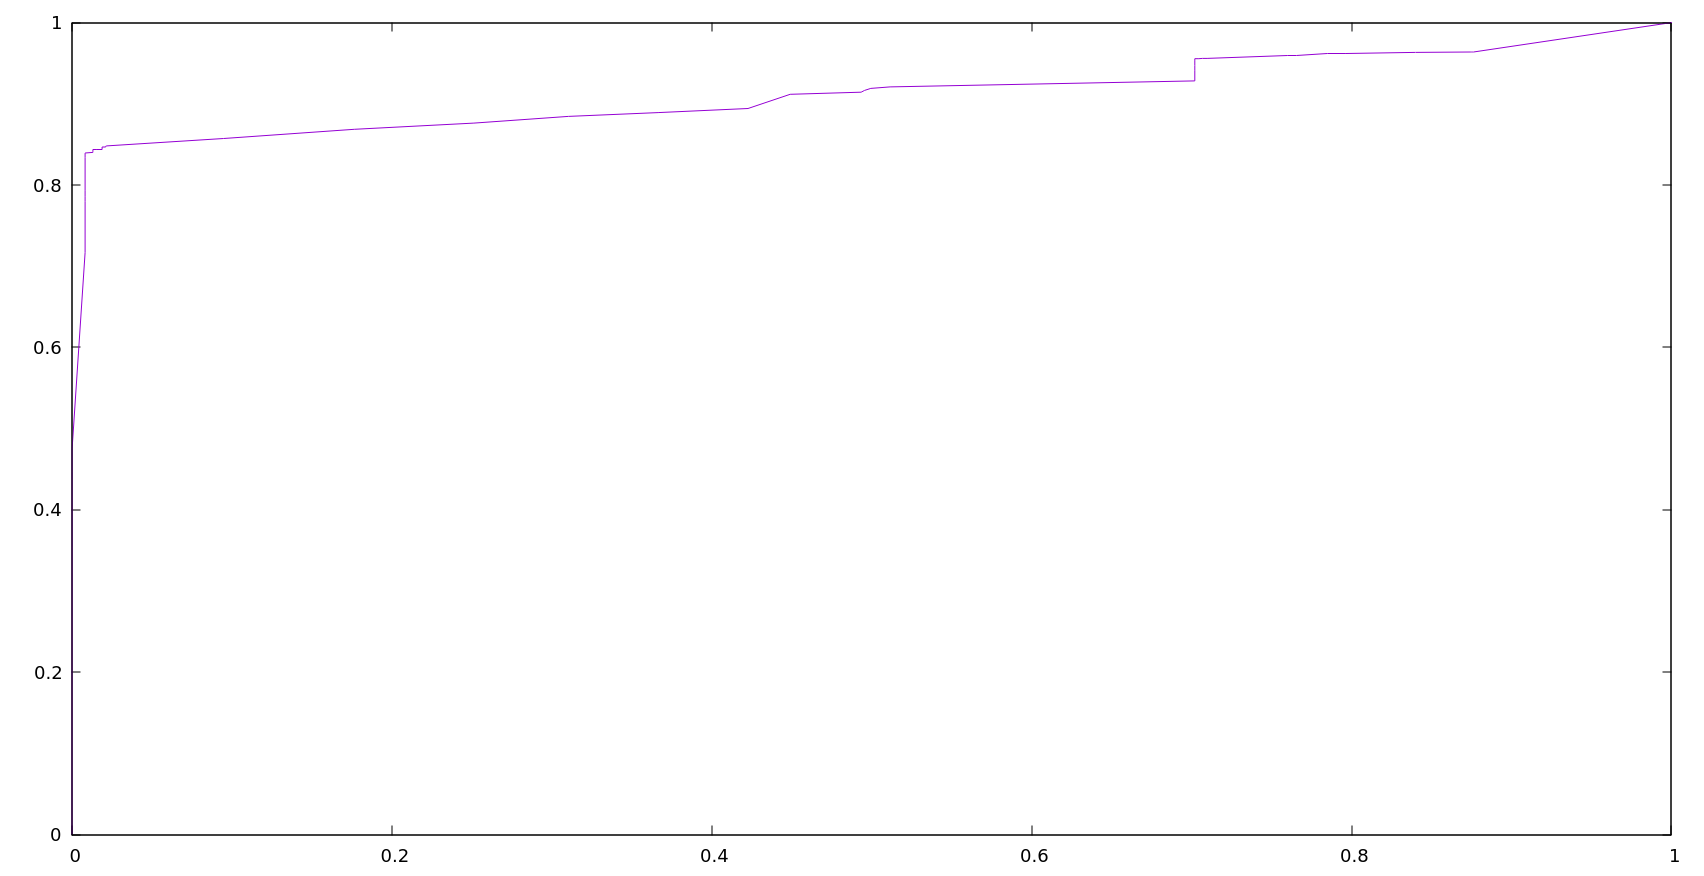
\includegraphics[scale=0.5]{roc1.png}
\caption{ROC Curve of Darpa Dataset After 60-Block Detections, AUC = 0.912}
\end{figure}

\begin{figure}[!ht]
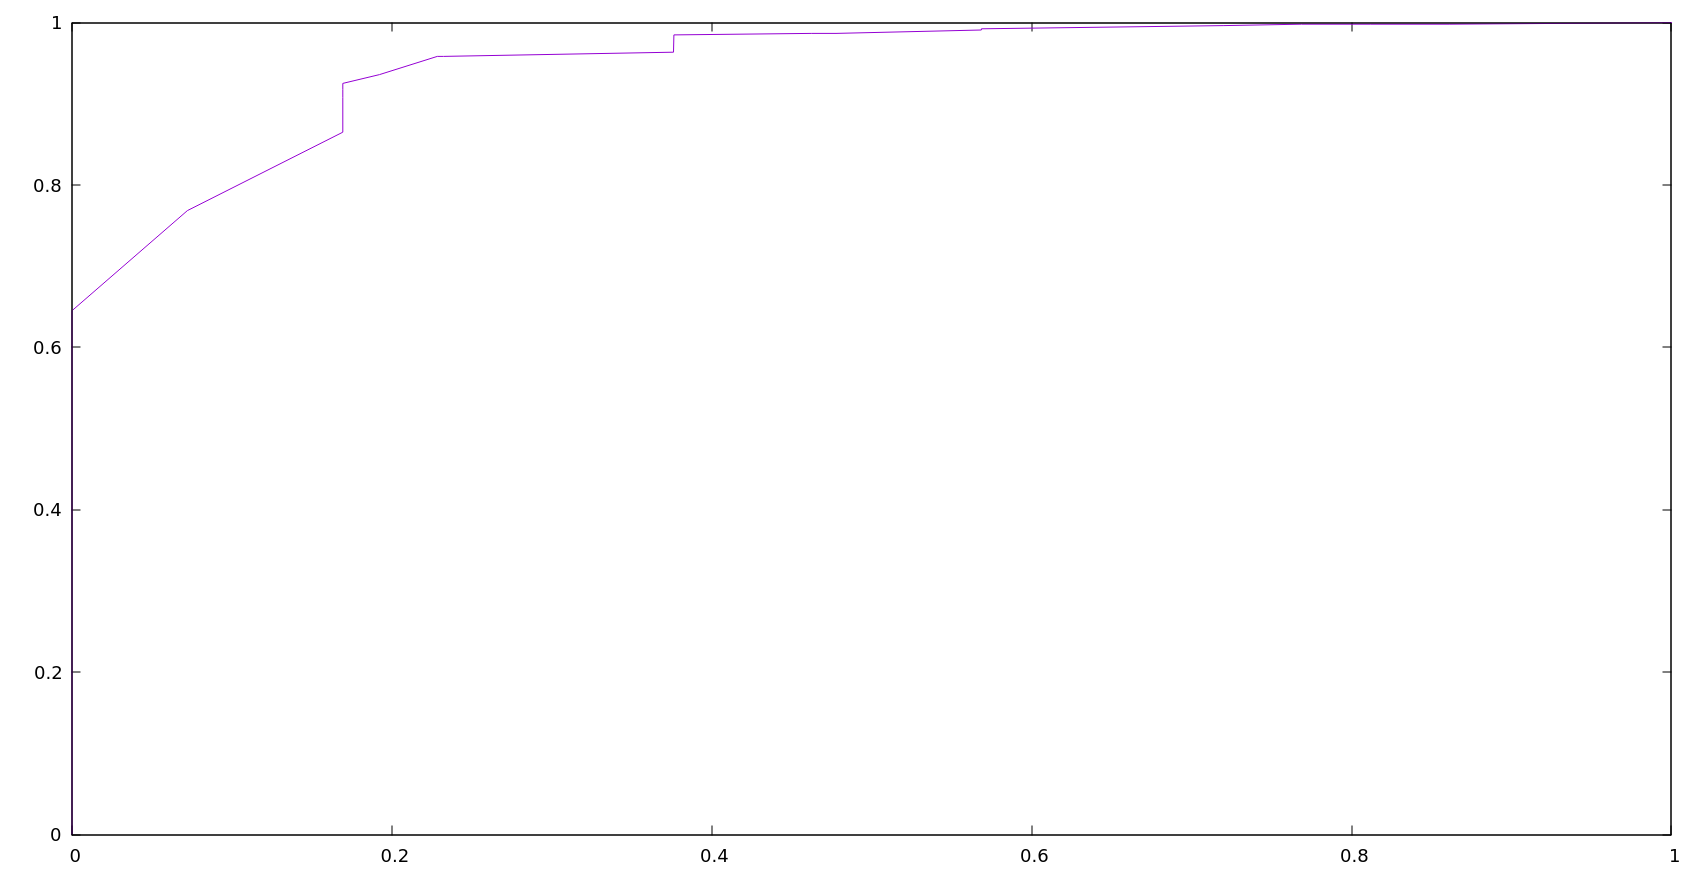
\includegraphics[scale=0.5]{roc2.png}
\caption{ROC Curve of Airforce Dataset After 20-Block Detections, AUC = 0.948}
\end{figure}
\paragraph{} From the ROC curves and AUC values we can see that the results we get on DARPA and AIRFORCE datasets are comparable to the
results presented in the original DCube paper. The true positive rate is way higher than false positive rate when number of blocks is small,
which means that our implementation can find the dense blocks which are most suspicious. The AUC values are also similar to the ones from the
original DCube paper. These results suggest that our SQL implementation can deliver results with comparable correctness on real-life datasets.
